\documentclass[ignorenonframetext,]{beamer}
\setbeamertemplate{caption}[numbered]
\setbeamertemplate{caption label separator}{: }
\setbeamercolor{caption name}{fg=normal text.fg}
\beamertemplatenavigationsymbolsempty
\usepackage{lmodern}
\usepackage{amssymb,amsmath}
\usepackage{ifxetex,ifluatex}
\usepackage{fixltx2e} % provides \textsubscript
\ifnum 0\ifxetex 1\fi\ifluatex 1\fi=0 % if pdftex
  \usepackage[T1]{fontenc}
  \usepackage[utf8]{inputenc}
\else % if luatex or xelatex
  \ifxetex
    \usepackage{mathspec}
  \else
    \usepackage{fontspec}
  \fi
  \defaultfontfeatures{Ligatures=TeX,Scale=MatchLowercase}
\fi
\usetheme[]{CambridgeUS}
\usecolortheme{beaver}
\usefonttheme{structurebold}
% use upquote if available, for straight quotes in verbatim environments
\IfFileExists{upquote.sty}{\usepackage{upquote}}{}
% use microtype if available
\IfFileExists{microtype.sty}{%
\usepackage{microtype}
\UseMicrotypeSet[protrusion]{basicmath} % disable protrusion for tt fonts
}{}
\newif\ifbibliography
\hypersetup{
            pdftitle={A3 The GESIS Panel data},
            pdfauthor={Kolb / Murray-Watters},
            pdfborder={0 0 0},
            breaklinks=true}
\urlstyle{same}  % don't use monospace font for urls
\usepackage{longtable,booktabs}
\usepackage{caption}
% These lines are needed to make table captions work with longtable:
\makeatletter
\def\fnum@table{\tablename~\thetable}
\makeatother
\usepackage{graphicx,grffile}
\makeatletter
\def\maxwidth{\ifdim\Gin@nat@width>\linewidth\linewidth\else\Gin@nat@width\fi}
\def\maxheight{\ifdim\Gin@nat@height>\textheight0.8\textheight\else\Gin@nat@height\fi}
\makeatother
% Scale images if necessary, so that they will not overflow the page
% margins by default, and it is still possible to overwrite the defaults
% using explicit options in \includegraphics[width, height, ...]{}
\setkeys{Gin}{width=\maxwidth,height=\maxheight,keepaspectratio}

% Prevent slide breaks in the middle of a paragraph:
\widowpenalties 1 10000
\raggedbottom

\AtBeginPart{
  \let\insertpartnumber\relax
  \let\partname\relax
  \frame{\partpage}
}
\AtBeginSection{
  \ifbibliography
  \else
    \let\insertsectionnumber\relax
    \let\sectionname\relax
    \frame{\sectionpage}
  \fi
}
\AtBeginSubsection{
  \let\insertsubsectionnumber\relax
  \let\subsectionname\relax
  \frame{\subsectionpage}
}

\setlength{\parindent}{0pt}
\setlength{\parskip}{6pt plus 2pt minus 1pt}
\setlength{\emergencystretch}{3em}  % prevent overfull lines
\providecommand{\tightlist}{%
  \setlength{\itemsep}{0pt}\setlength{\parskip}{0pt}}
\setcounter{secnumdepth}{0}

\title{A3 The GESIS Panel data}
\author{Kolb / Murray-Watters}
\date{06 August 2018}

\begin{document}
\frame{\titlepage}

\begin{frame}{Das GESIS Panel}

\begin{itemize}
\tightlist
\item
  Wahrscheinlichkeitsbasiertes Access Panel für Individuen: - Allgemeine
  Bevölkerung in Deutschland, Deutschsprachhige Bevölkerung, 18-70 Jahre
\item
  Panelisten wurden aus den Melderegistern rekrutiert - (270 Sampling
  Points) 7599 face-to-face Interviews (CAPI)
\item
  Ungefähr 5000 Panelisten (Basis Stichprobe / erste Kohorte 2014)
\end{itemize}

\end{frame}

\begin{frame}{Das GESIS Panel Campus File}


\includegraphics{figure/gpdata.PNG}

\end{frame}

\begin{frame}[fragile]{Download data}

\begin{itemize}
\tightlist
\item
  Übersichtsseite:
  \href{https://www.gesis.org/gesis-panel/data/gesis-panel-campus-file/}{\textbf{GESIS
  Panel Campus File}}
\item
  Registrierung notwendig
\end{itemize}

\begin{block}{Links für den Download:}

\begin{itemize}
\tightlist
\item
  \href{https://dbk.gesis.org/dbksearch/download.asp?db=D\&id=62367}{\textbf{Download
  \texttt{.csv}}}
\item
  \href{https://dbk.gesis.org/dbksearch/download.asp?db=D\&id=62369}{\textbf{Download
  \texttt{.sav}}}
\item
  \href{https://dbk.gesis.org/dbksearch/download.asp?db=D\&id=62371}{\textbf{Download
  \texttt{**14.dta}}}
\end{itemize}

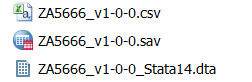
\includegraphics{figure/filenamesGP2.PNG}

\end{block}

\end{frame}

\begin{frame}{Einen ersten Eindruck von den Daten bekommen}

\begin{itemize}
\tightlist
\item
  bbzc022a - Häufigkeit politische Nachrichten
\item
  bfam051a - MPMB Capacity: Termine fallen rechtzeitig ein
\item
  bfzi023a - Umfragen GESIS GM: Interessant
\item
  baai124a - Schwierigkeit Fragebogen zu verstehen
\end{itemize}

\begin{longtable}[]{@{}llll@{}}
\toprule
bbzc022a & bfam051a & bfzi023a & baai124a\tabularnewline
\midrule
\endhead
Täglich weniger als eine Stunde & Eher selten & 7 Stimme voll und ganz
zu & Etwas schwierig\tabularnewline
Täglich weniger als eine Stunde & Eher oft & 6 & Überhaupt nicht
schwierig\tabularnewline
Täglich weniger als eine Stunde & Eher selten & 2 & Etwas
schwierig\tabularnewline
Einmal im Monat oder seltener & Eher oft & 7 Stimme voll und ganz zu &
Überhaupt nicht schwierig\tabularnewline
Täglich weniger als eine Stunde & Eher oft & 3 & Überhaupt nicht
schwierig\tabularnewline
Einmal in der Woche & Not reached & 4 & Etwas schwierig\tabularnewline
\bottomrule
\end{longtable}

\end{frame}

\begin{frame}[fragile]{Die Variablennamen im GESIS Panel}

\begin{block}{Beispiel für die Zusammensetzung der Variablennamen}

\begin{verbatim}
## [1] "bezf044a" "bdze018a" "bdao036b" "bfzi029a" "bezg091a"
\end{verbatim}

\begin{itemize}
\tightlist
\item
  Die ersten beiden Buchstaben enthalten die Welle:
\end{itemize}

\begin{longtable}[]{@{}rll@{}}
\toprule
year & waves & numbers\tabularnewline
\midrule
\endhead
2013 & aa,ab,ac,ad,ae,af & 1-6\tabularnewline
2014 & ba,bb,bc,bd,be,bf & 7-12\tabularnewline
2015 & ca,cb,cc,cd,ce,cf & 13-18\tabularnewline
2016 & da,db,dc,dd,de,df & 19-24\tabularnewline
2017 & ea,eb,ec,ed,ee,ef & 25-30\tabularnewline
2018 & fa,fb,fc,fd,fe,ff & 31-36\tabularnewline
\bottomrule
\end{longtable}

\begin{itemize}
\tightlist
\item
  Bis zum jetzigen Zeitpunkt sind 34 gelaufen
\end{itemize}

\end{block}

\end{frame}

\begin{frame}{Die Variablennamen im GESIS Panel II}

\begin{itemize}
\tightlist
\item
  Die Stellen drei und vier geben Information über die Studie:
\end{itemize}

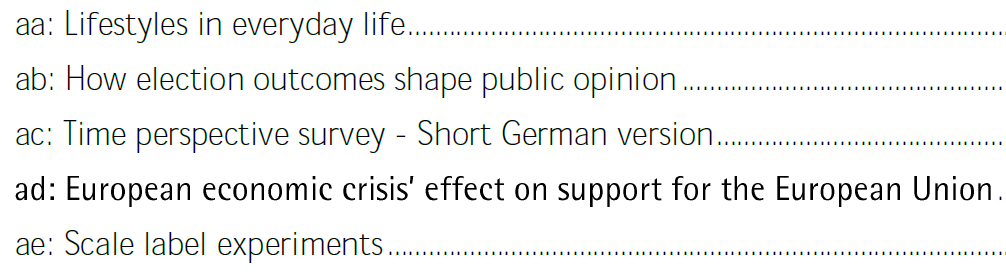
\includegraphics{figure/examplestudies.PNG}

\begin{itemize}
\item
  Die Stellen fünf, sechs und sieben indizieren die Variablennummer
\item
  Die letzte Stelle enthält die Information, ob es sich um eine
  originale Variable (a) oder eine synthetische Variable handelt
  (b,c,d,e,\ldots{})
\end{itemize}

\end{frame}

\begin{frame}[fragile]{Variablennamen im GESIS Panel}

\begin{block}{Beispiel Geburtsdatum - \texttt{cfzh072c}}

\begin{verbatim}
## [1] "cfzh072c"
\end{verbatim}

\begin{verbatim}
## [1] "Welle:  cf"
\end{verbatim}

\begin{verbatim}
## [1] "Studie:  zh"
\end{verbatim}

\begin{verbatim}
## [1] "Variablen Nr.:  072"
\end{verbatim}

\begin{verbatim}
## [1] "Synthetische Variable?:  c"
\end{verbatim}

\end{block}

\end{frame}

\begin{frame}{Die Variablen im Campus File}

\url{https://rpubs.com/Japhilko82/VarsGesisPanel}

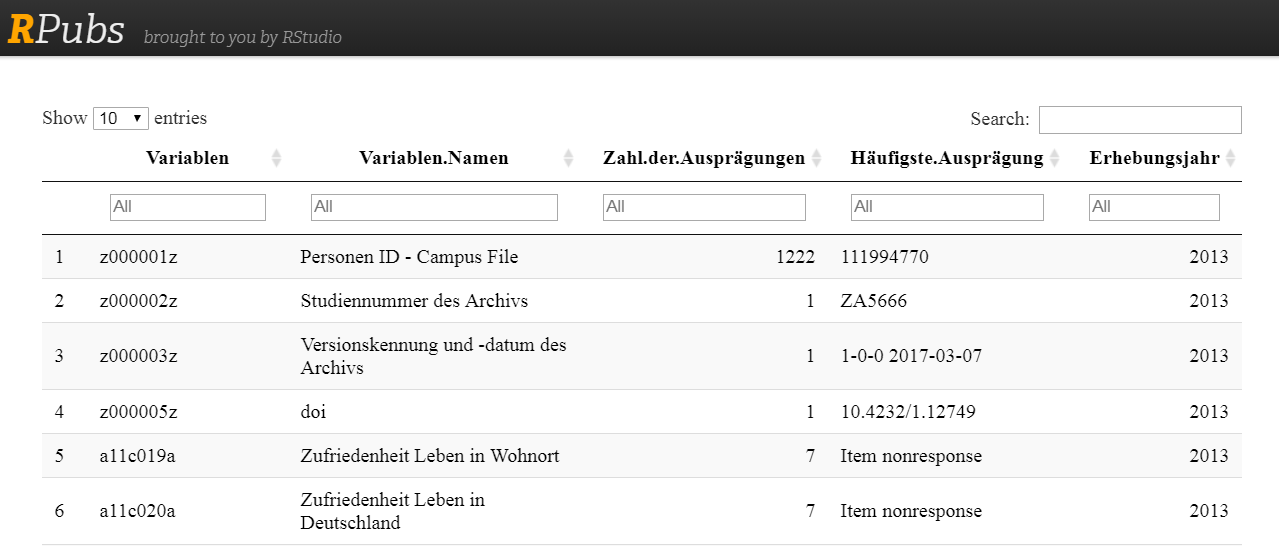
\includegraphics{figure/rpubs_varspuf.PNG}

\end{frame}

\begin{frame}[fragile]{Wellen im Campus File}

\begin{itemize}
\tightlist
\item
  Welche Wellen sind im Campus file?
\item
  Anzahl Variablen pro Welle im Campus File:
\end{itemize}

\begin{verbatim}
## waves
##  a1  ba  bb  bc  bd  be  bf  z0 
## 171 171 154 155 224 185 128   4
\end{verbatim}

\end{frame}

\begin{frame}{Die Missing Codes im GESIS Panel}

\begin{longtable}[]{@{}rll@{}}
\toprule
Value & Value.label & Remark\tabularnewline
\midrule
\endhead
-11 & Not invited & only in recruitment waves as long as the respective
profile survey is not yet finished\tabularnewline
-22 & Not in panel & not willing to join the panel after recruitment
interview or actively signing off the panel\tabularnewline
-33 & Unit nonresponse & invited but not participating in corresponding
wave\tabularnewline
-44 & Missing by m.o.p. & mode of participation (m.o.p.): online or
offline\tabularnewline
-55 & Missing by technical error & e.g.~questionnaire programming
error\tabularnewline
-66 & Missing by design & experimental variation\tabularnewline
-77 & Not reached & only in online mode: panelist has not seen the
item\tabularnewline
-88 & Missing by filter & filtered item\tabularnewline
-99 & Item nonresponse & due to nonresponse by the
respondent\tabularnewline
-111 & Ambiguous answer & ambiguous answers in
questionnaire\tabularnewline
\bottomrule
\end{longtable}

\end{frame}

\begin{frame}{Satisfaction life in place of residence (a11c019a)}

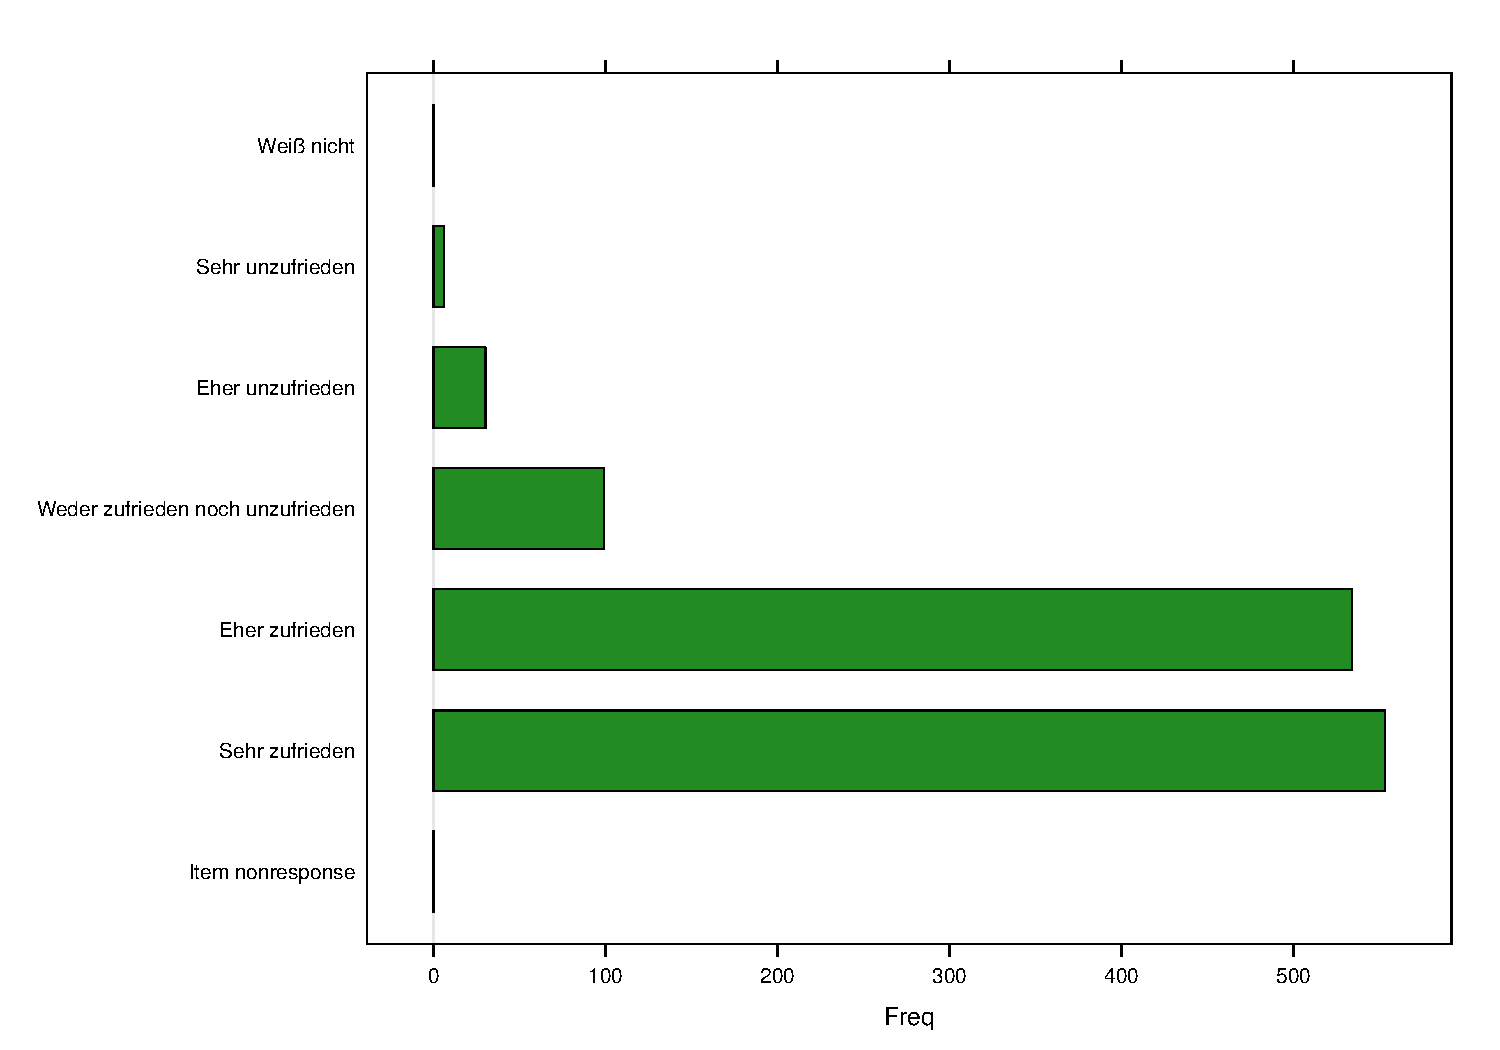
\includegraphics{A3_GESISPanel_files/figure-beamer/unnamed-chunk-17-1.pdf}

\end{frame}

\begin{frame}{The codebook}

\begin{itemize}
\tightlist
\item
  You can get the codebook
  \href{https://www.gesis.org/gesis-panel/documentation/}{\textbf{here}}
\end{itemize}

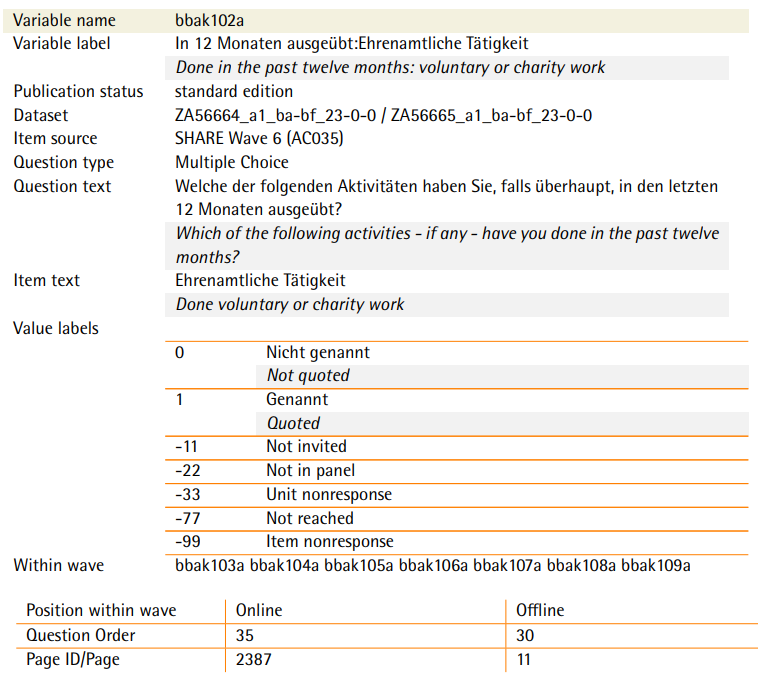
\includegraphics{figure/cdb_bbak102a.PNG}

\end{frame}

\begin{frame}[fragile]{A3A Exercise - Downloading the GESIS Panel data}

\begin{itemize}
\tightlist
\item
  Please download \texttt{.csv}, \texttt{.sav} and \texttt{**14.dta} of
  the GESIS Panel Campus file.
\end{itemize}

\end{frame}

\end{document}
